\documentclass{standalone}

\usepackage{tikz}
\usetikzlibrary{calc, intersections}


\begin{document}
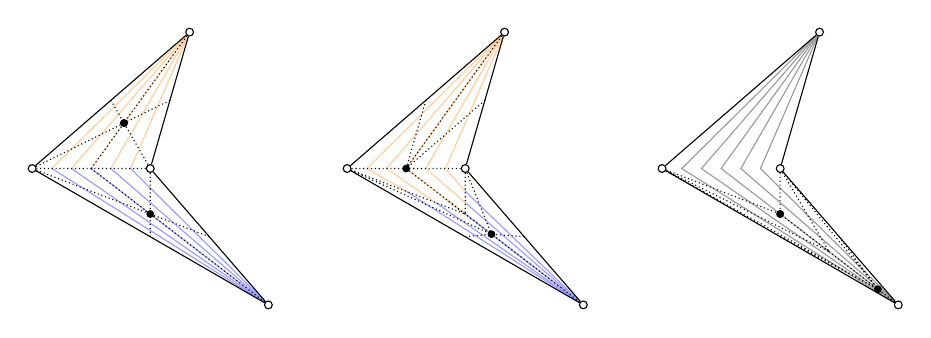
\begin{tikzpicture}[scale=2]
  \pgfmathsetmacro{\y}{sqrt(3)/2}
  \pgfmathsetmacro{\xl}{1/2}

  \def\setup{
    % Name the vertices of the simplex
    % a
    % / \
    % c - b
    % \ /
    % d
    %
    \node[circle, draw=black, fill=white, inner sep=1pt] (a) at (\xl,\y) {};
    \node[circle, draw=black, fill=white, inner sep=1pt] (b) at (\xl/2,0) {};
    \node[circle, draw=black, fill=white, inner sep=1pt] (c) at (-\xl,0) {};
    \node[circle, draw=black, fill=white, inner sep=1pt] (d) at (2*\xl,-\y) {};
    \coordinate (mab) at ($.5*(a) + .5*(b)$);
    \coordinate (mac) at ($.5*(a) + .5*(c)$);
    \coordinate (mbd) at ($.5*(d) + .5*(b)$);
    \coordinate (mcd) at ($.5*(d) + .5*(c)$);

    \coordinate (baanc) at (0.0, 0.28867513459481287);
    \coordinate (bbanc) at (0.0, -0.8660254037844386);
  }

  \def\drawss{


    \draw[densely dotted] (a) -- (b1) (b) -- (b1) (c) -- (b1) (mab) -- (b1)
    (mac) -- (b1) (mbc) -- (b1) (b) -- (mbc) -- (c);

    \draw[densely dotted] (d) -- (b2) (b) -- (b2) (c) -- (b2) (mbd) -- (b2)
    (mcd) -- (b2) (mbc) -- (b2);

    % Draw boundary of simplex
    \draw (a) -- (b) -- (d) -- (c) -- (a);


  }

  % Start point and endpoint
  \coordinate (spoint) at (0.08333333333, .288675) {};
  \coordinate (epoint) at (.25, -.288675) {};

  % Number of auxilliary lines to draw
  \pgfmathsetmacro{\numaux}{5}
  \pgfmathsetmacro{\halfaux}{(\numaux+1)/2}
  \pgfmathsetmacro{\halfauxplus}{\halfaux+1}

  \begin{scope}[xshift=-2cm]
    \coordinate (sspoint) at ($(spoint) + (-2.,0.)$);
    \node[circle, fill=black, inner sep=1pt] (dpoint) at ($(sspoint) +
    (0.,0.)$) {};

    \coordinate (b1) at (0.08333333333, .288675);
    \coordinate (b2) at (.25, -.288675) {};

    \setup

    \coordinate (mbc) at ($.5*(b) + .5*(c)$);

    \foreach \rat in {1,2,3,...,\numaux}{
      \pgfmathsetmacro{\ratfrac}{\rat/(\numaux+1)}
      \pgfmathsetmacro{\compratf}{1 - \ratfrac}

      \coordinate (bc\rat) at ($\ratfrac*(b) + \compratf*(c)$);

      \draw[orange!40!white] (a) -- (bc\rat);
      \draw[blue!40!white] (d) -- (bc\rat);
    }

    \drawss

    \node[circle, fill=black, inner sep=1pt] () at (b1) {};
    \node[circle, fill=black, inner sep=1pt] () at (b2) {};


  \end{scope}

  \begin{scope}[xshift=0cm]
    \coordinate (sspoint) at (spoint);
    \coordinate (dpoint) at ($.5*(spoint) + .5*(epoint)$);

    \coordinate (b1) at (-.125, 0);
    \coordinate (b2) at (.41666666, -.416975) {};

    \setup

    \coordinate (mbc) at ($.5*(b1) + .5*(b2)$);

    \foreach \rat in {1,2,3,...,\halfaux}{
      \pgfmathsetmacro{\ratfrac}{\rat/(\numaux+1)}
      \pgfmathsetmacro{\compratf}{1 - \ratfrac}

      \coordinate (bc\rat) at ($\ratfrac*(b) + \compratf*(c)$);

      \pgfmathsetmacro{\rfa}{(\rat+1)/(\numaux+1)}
      \pgfmathsetmacro{\crfa}{1 - \rfa}

      \draw[orange!40!white] (a) -- (bc\rat) -- ($\rfa*(mbd) + \crfa*(c)$);
      \draw[blue!40!white] ($\rfa*(mbd) + \crfa*(c)$) -- (d);
    }

    \foreach \rat in {\halfaux,..., \numaux}{
      \pgfmathsetmacro{\ratfrac}{\rat/(\numaux+1)}
      \pgfmathsetmacro{\compratf}{1 - \ratfrac}

      \coordinate (bc\rat) at ($\ratfrac*(b) + \compratf*(c)$);

      \pgfmathsetmacro{\rfa}{(\rat-1)/(\numaux+1)}
      \pgfmathsetmacro{\crfa}{1 - \rfa}

      \draw[orange!40!white] (a) -- (bc\rat) -- ($\rfa*(b) + \crfa*(mcd)$);
      \draw[blue!40!white] ($\rfa*(b) + \crfa*(mcd)$) -- (d);
    }


    \draw[densely dotted] (a) -- (b1) (b) -- (b1) (c) -- (b1) (mab) -- (b1)
    (mac) -- (b1) (epoint) -- (b1) (b) -- (epoint) -- (c);

    \draw[densely dotted] (d) -- (b2) (b) -- (b2) (c) -- (b2) (mbd) -- (b2)
    (mcd) -- (b2) (mbc) -- (b2);

    % Draw boundary of simplex
    \draw (a) -- (b) -- (d) -- (c) -- (a);

    \node[circle, fill=black, inner sep=1pt] () at (b1) {};
    \node[circle, fill=black, inner sep=1pt] () at (b2) {};

  \end{scope}

  \begin{scope}[xshift=2cm]
    \coordinate (sspoint) at ($(spoint) + (2.,0.)$);
    \coordinate (epoint) at ($(epoint) + (2., 0)$);
    \node[circle, fill=black, inner sep=1pt] (dpoint) at
    (epoint) {};

    \coordinate (b1) at (dpoint);
    \coordinate (b2) at (.870370, -.766236);

    \setup
    \coordinate (mbc) at ($.5*(b1) + .5*(b2)$);


    \foreach \rat in {1,2,3,...,\numaux}{
      \pgfmathsetmacro{\ratfrac}{\rat/(\numaux+1)}
      \pgfmathsetmacro{\compratf}{1 - \ratfrac}

      \coordinate (bc\rat) at ($\ratfrac*(b) + \compratf*(c)$);

      \pgfmathsetmacro{\rfa}{(\rat+1)/(\numaux+1)}
      \pgfmathsetmacro{\crfa}{1 - \rfa}

      \draw[black!40!white] (a) -- (bc\rat) -- (d);
    }

    \foreach \rat in {\halfaux,..., \numaux}{
      \pgfmathsetmacro{\ratfrac}{\rat/(\numaux+1)}
      \pgfmathsetmacro{\compratf}{1 - \ratfrac}

      \coordinate (bc\rat) at ($\ratfrac*(b) + \compratf*(c)$);

      \pgfmathsetmacro{\rfa}{(\rat-1)/(\numaux+1)}
      \pgfmathsetmacro{\crfa}{1 - \rfa}
    }


    \draw[densely dotted] % (a) -- (b1)
    (b) -- (b1) (c) -- (b1) % (mab) -- (b1)
    % (mac) -- (b1)
    (mbc) -- (b1) (b) -- (mbc) -- (c);

    \draw[densely dotted] (d) -- (b2) (b) -- (b2) (c) -- (b2) (mbd) -- (b2)
    (mcd) -- (b2) (mbc) -- (b2);

    % Draw boundary of simplex
    \draw (a) -- (b) -- (d) -- (c) -- (a);



    \node[circle, fill=black, inner sep=1pt] () at (b1) {};
    \node[circle, fill=black, inner sep=1pt] () at (b2) {};

  \end{scope}
\end{tikzpicture}
\end{document}
